% vim: set fileencoding=utf-8:
\documentclass{beamer}
\usepackage[utf8]{inputenc}
\usepackage[spanish]{babel}
\usepackage{fancybox}
\usepackage{graphics}
\usepackage{xcolor}
\usepackage{amsmath}
\usepackage{wasysym}

\usecolortheme{crane}
\setbeamercovered{transparent}
%\includeonlyframes{current}

\newcommand{\key}[1]{%
    \fcolorbox{black}{lightgray}{\rule[-.2em]{0pt}{1em}\makebox[1em][l]{#1}}%
}
\newcommand{\longkey}[1]{%
    \fcolorbox{black}{lightgray}{\rule[-.2em]{0pt}{1em}\makebox{#1}}%
}
\newcommand{\anykey}{%
    \fcolorbox{black}{red!75!green!50}{\rule[-.2em]{0pt}{1em}\makebox[1em][l]{}}%
}
\newcommand{\cmd}[1]{%
    \fcolorbox{black}{blue!75!green!50}{\rule[-.2em]{0pt}{1em}\makebox{\emph{#1}}}%
}
\newcommand{\cmdcount}{%
    \fcolorbox{black}{red!45!yellow!25}{\rule[-.2em]{0pt}{1em}\makebox{\emph{count}}}%
}
\newcommand{\typed}[1]{%
    \fcolorbox{blue!25!green!75}{blue!25!green!75}{\rule[-.2em]{0pt}{1em}\makebox{\texttt{#1}}}%
}
\newcommand{\placeholder}[1]{ \emph{$\langle$#1$\rangle$} }
\newcommand{\good}{ \textcolor{blue!25!green!75}{\Large\smiley} }
\newcommand{\bad}{ \textcolor{red}{\Large\frownie} }
\newcommand{\foreign}{\textit}

\title {Edición eficiente de texto con Vim}
\author{Roberto Bonvallet \\ $\langle$rbonvall@inf.utfsm.cl$\rangle$}
\institute[UTFSM]{ Departamento de Informática \\
    Universidad Técnica Federico Santa María }
\date{20 de agosto de 2009}

\begin{document}

%\begin{frame}
%    \includegraphics[width=2in]{vim_putz1.jpg}
%    \includegraphics[width=2in]{vim_putz2.jpg}
%\end{frame}

\begin{frame}
    \titlepage
\end{frame}

\begin{frame}
    \begin{block}{Diapos}
        \large git~clone~\textbf{git:/\!\!/github.com/rbonvall/charla-vim.git}
    \end{block}
    \begin{block}{Reutilice a su antojo}
        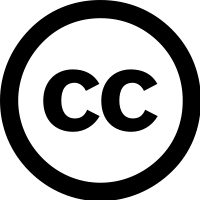
\includegraphics[width=1in]{cc}
        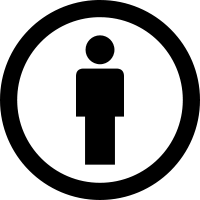
\includegraphics[width=1in]{cc-by}
        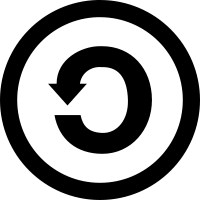
\includegraphics[width=1in]{cc-sa}
    \end{block}
\end{frame}

\begin{frame}
    \only<1>{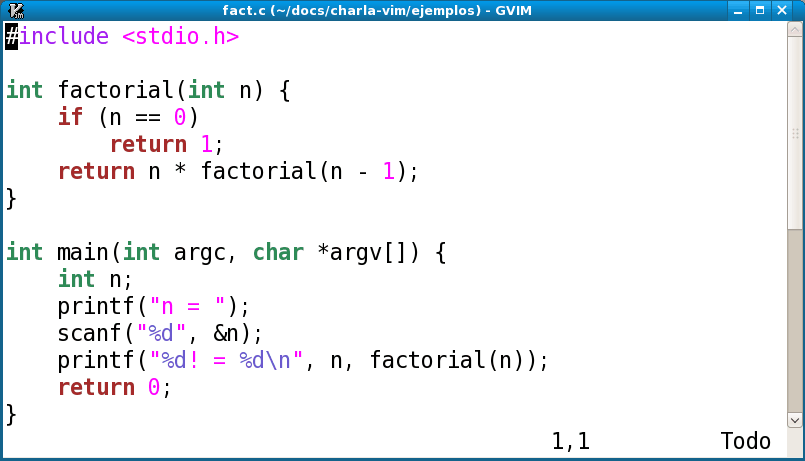
\includegraphics[width=\textwidth]{capturas/fact-01-nq8}}
    \only<2>{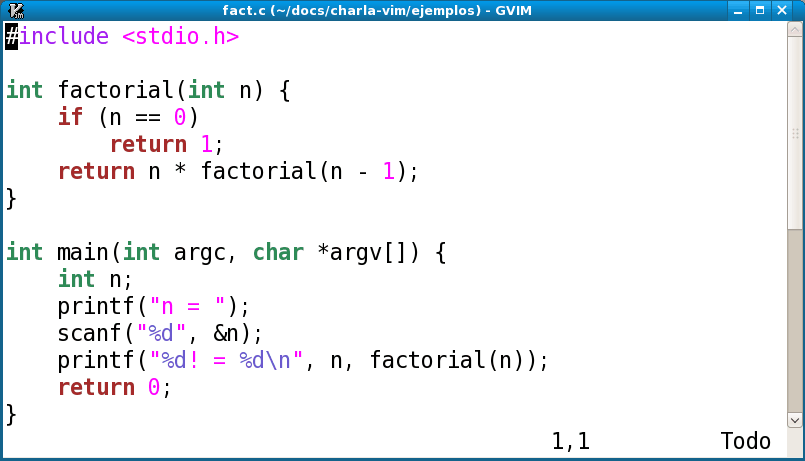
\includegraphics[width=\textwidth]{capturas/fact-02-nq8}}
    \only<3>{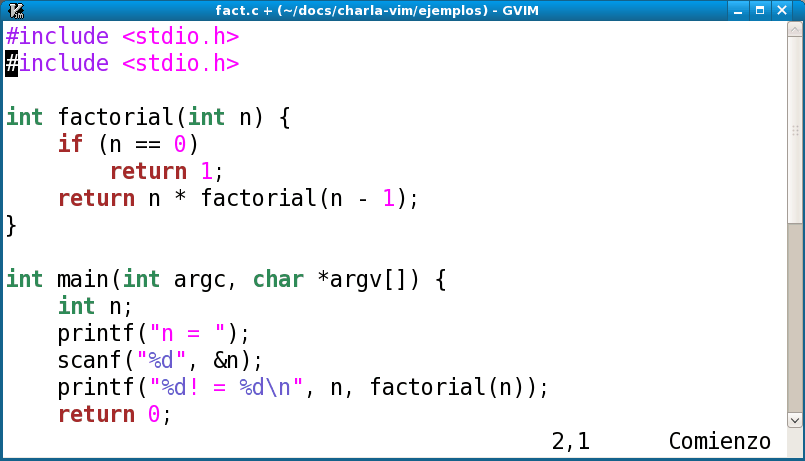
\includegraphics[width=\textwidth]{capturas/fact-03-nq8}}
    \only<4>{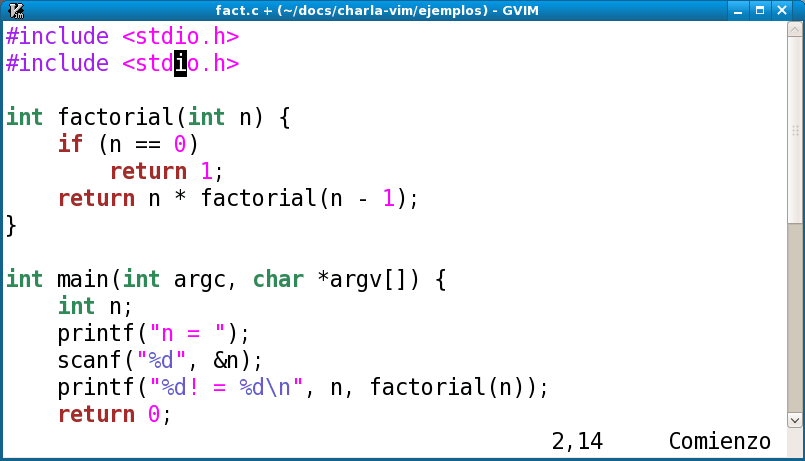
\includegraphics[width=\textwidth]{capturas/fact-04-nq8}}
    \only<5>{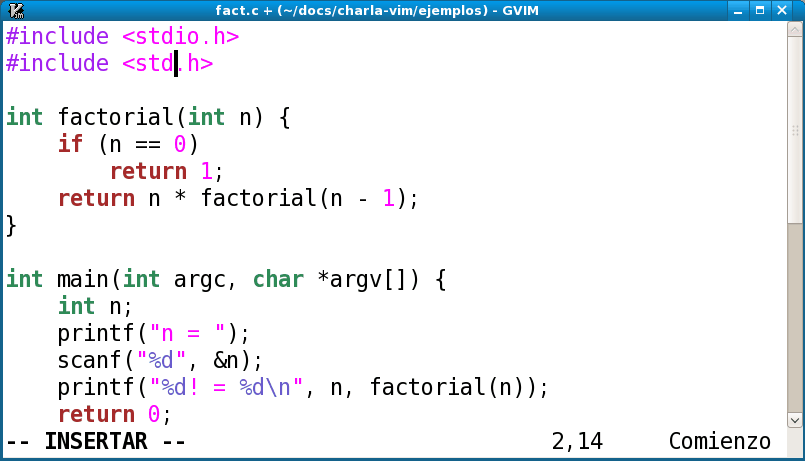
\includegraphics[width=\textwidth]{capturas/fact-05-nq8}}
    \only<6>{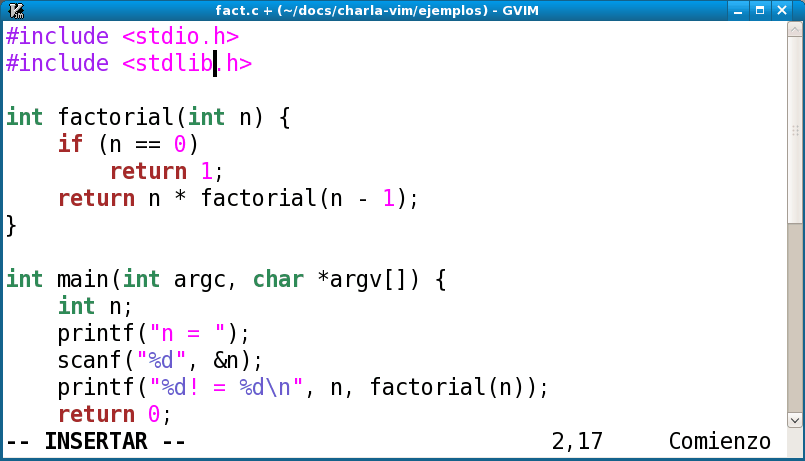
\includegraphics[width=\textwidth]{capturas/fact-06-nq8}}
    \only<7>{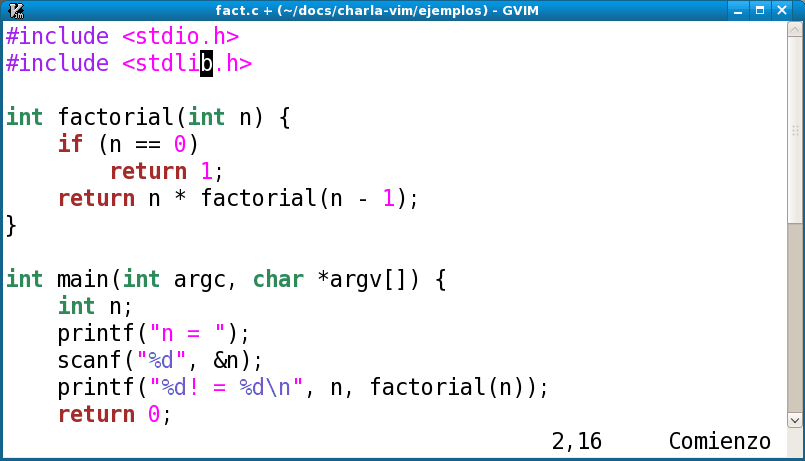
\includegraphics[width=\textwidth]{capturas/fact-07-nq8}}
    \only<8>{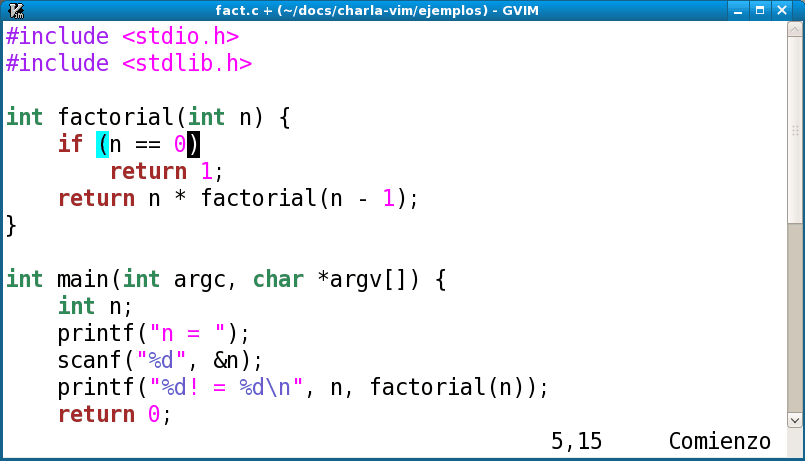
\includegraphics[width=\textwidth]{capturas/fact-08-nq8}}
    \only<9>{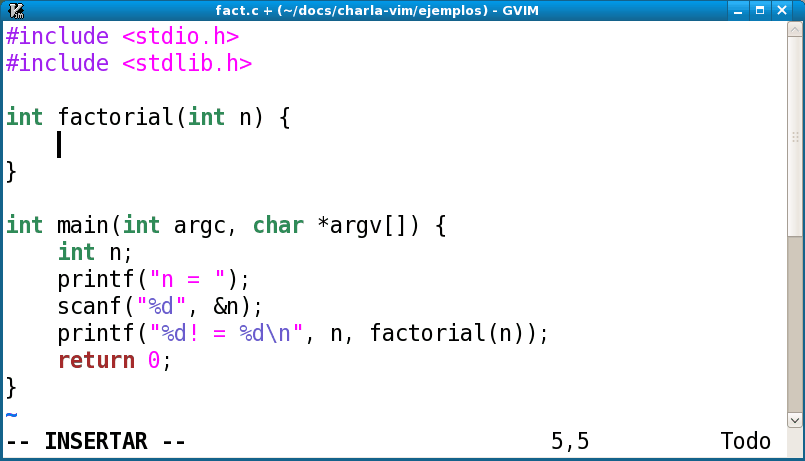
\includegraphics[width=\textwidth]{capturas/fact-09-nq8}}
    \only<10>{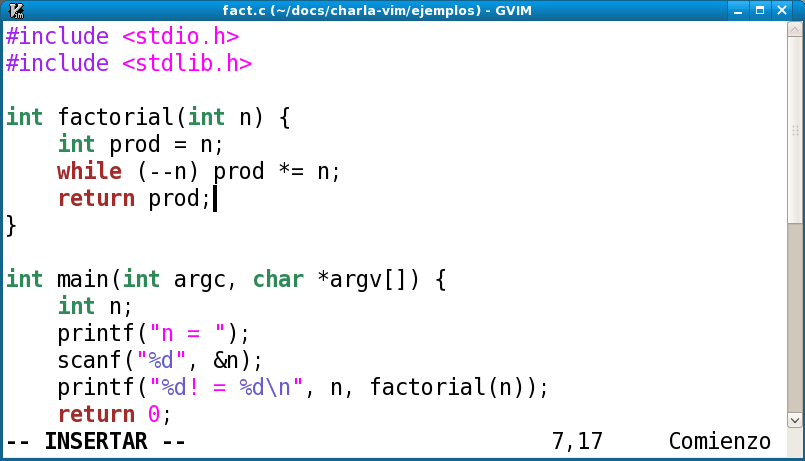
\includegraphics[width=\textwidth]{capturas/fact-10-nq8}}
    \only<11>{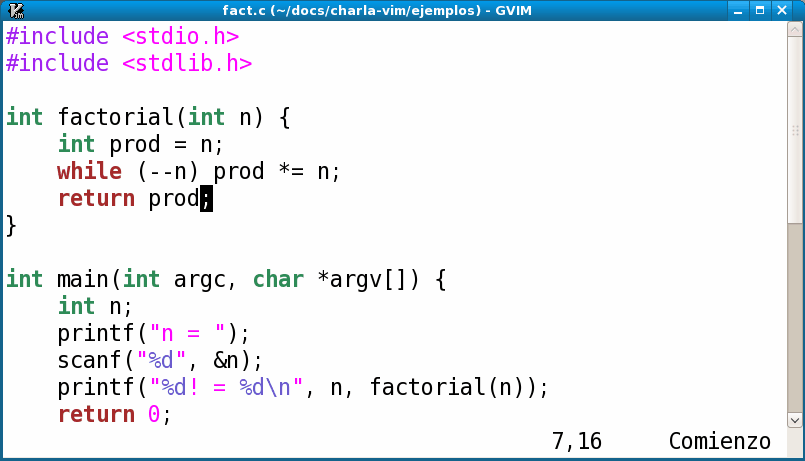
\includegraphics[width=\textwidth]{capturas/fact-11-nq8}}
    \only<12>{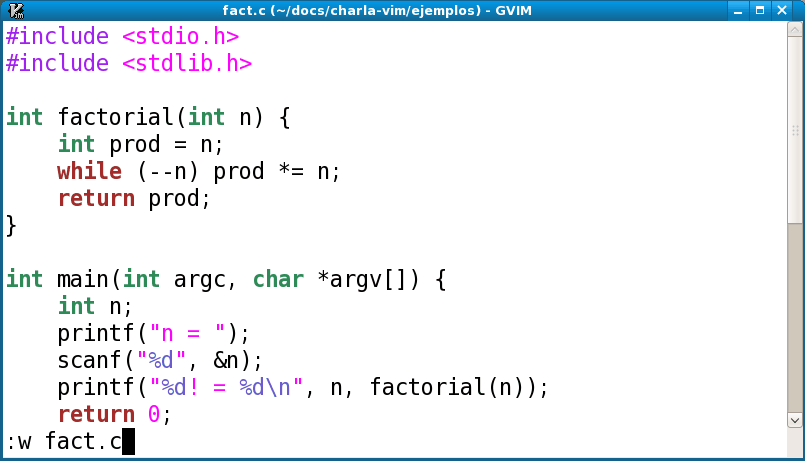
\includegraphics[width=\textwidth]{capturas/fact-12-nq8}}
    \only<13>{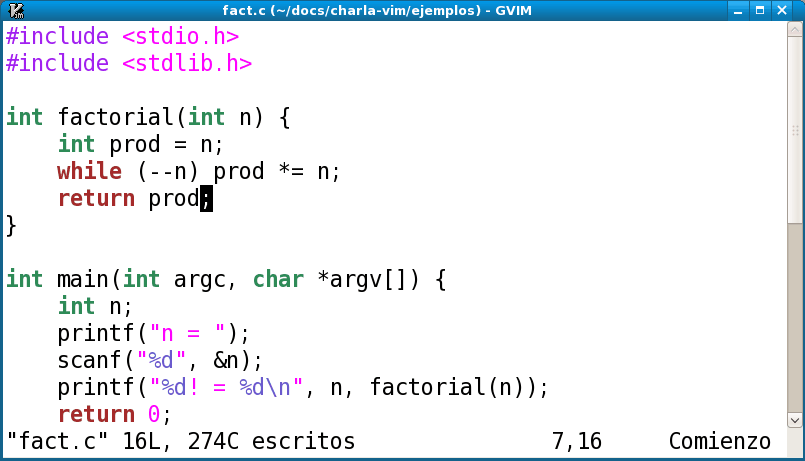
\includegraphics[width=\textwidth]{capturas/fact-13-nq8}}
    \only<14>{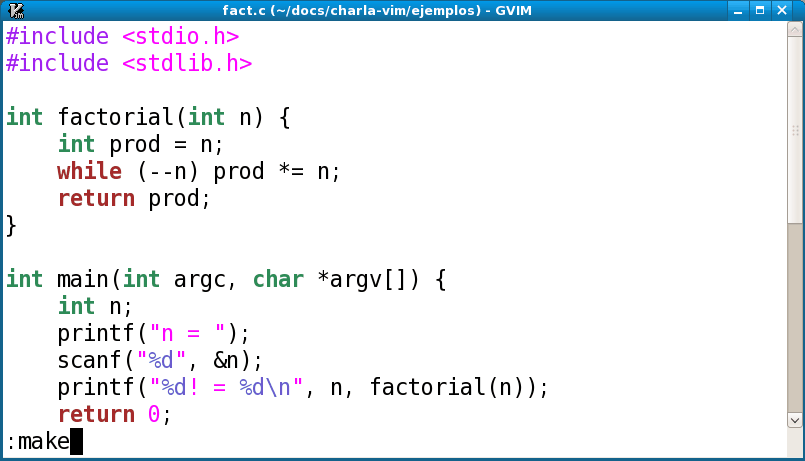
\includegraphics[width=\textwidth]{capturas/fact-14-nq8}}
    \only<15>{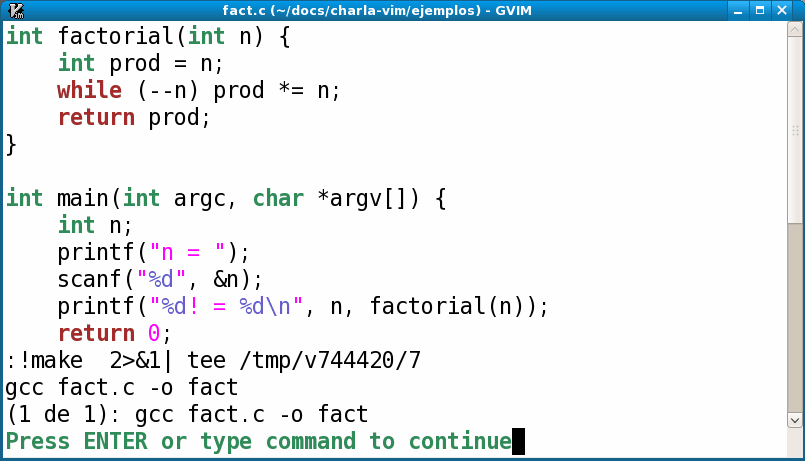
\includegraphics[width=\textwidth]{capturas/fact-15-nq8}}
    \uncover<2->{\key{y}\key{y}}
    \uncover<3->{\key{p}}
    \uncover<4->{\key{2}\key{f}\key{i}}
    \uncover<5->{\key{c}\key{w}}
    \uncover<6->{\typed{lib}}%
    \uncover<7->{\longkey{Esc}}
    \uncover<8->{\key{3}\key{j}} \\
    \uncover<9->{\key{c}\key{i}\key{$\}$}}
    \uncover<10->{\ldots}%
    \uncover<11->{\longkey{Esc}}
    \uncover<12->{\key{:}\typed{w fact.c}}%
    \uncover<13->{\longkey{Enter}}
    \uncover<14->{\key{:}\typed{make}}%
    \uncover<15->{\longkey{Enter}}
\end{frame}

\begin{frame}
    \frametitle{Utilización del teclado}
    \only<1>{
        \begin{figure}[h]
            \begin{center}
                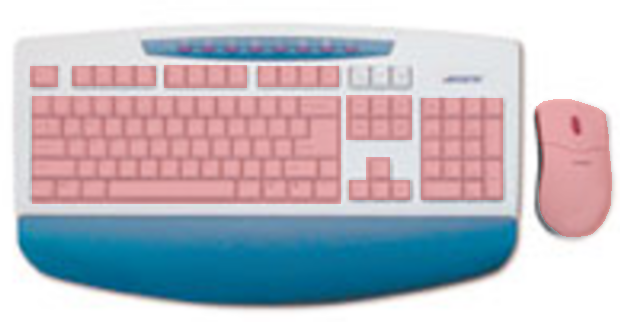
\includegraphics[width=4in]{kb-use-common}
            \end{center}
            \caption{à la Bloc de Notas}
            \label{fig:kb-use-common}
        \end{figure}
    }
    \only<2>{
        \begin{figure}[h]
            \begin{center}
                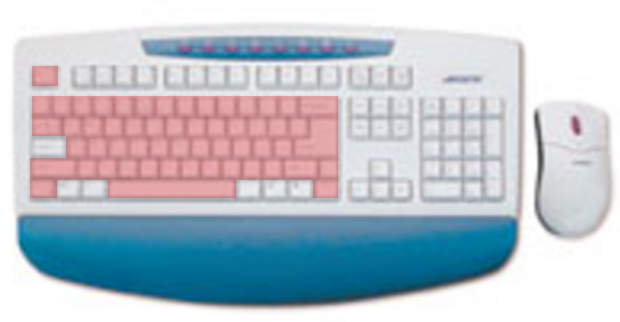
\includegraphics[width=4in]{kb-use-vim}
            \end{center}
            \caption{à la Vim}
            \label{fig:kb-use-vim}
        \end{figure}
    }
\end{frame}

\begin{frame}
    \frametitle{Notación}
    \begin{itemize}
        \item \key{$x$}: la tecla $x$ presionada
        \item \anykey: una tecla cualquiera presionada
        \item \cmd{mov}: un movimiento realizado
        \item \cmdcount: un número tipeado antes de un comando
        \item \typed{lala}: el texto \textit{lala} tipeado tal cual
    \end{itemize}
\end{frame}

\begin{frame}
    \frametitle{Los comandos más paltosos del mundo}
    \begin{itemize}
        \item \key{.}: repite el último comando
        \item \key{u}: deshace el último comando (\foreign{undo})
        \item \longkey{Ctrl R}: rehace lo deshecho (\foreign{redo})
    \end{itemize}
\end{frame}

\begin{frame}
    \frametitle{Movimientos \cmd{\hspace{1.5em}}}
    \begin{itemize}
        \item \good \key{h}, \key{j}, \key{k}, \key{l} =
              \bad \key{$\leftarrow$}, \key{$\downarrow$},
                 \key{$\uparrow$}, \key{$\rightarrow$}.
        \item \key{w}, \key{b}, \key{e}:
            \foreign{word}, \foreign{beginning of word}, \foreign{end of word}.
        \item \key{0}, \key{\$}: comienzo, final de línea
        \item \key{g}\key{g}, \key{G}: comienzo, final del archivo
        \item \key{f}\anykey, \key{F}\anykey:
            siguiente, anterior ``\anykey{}'' (\foreign{find})
        \item \key{\%}: aparea paréntesis
        \item \key{$($}, \key{$)$}, \key{\{}, \key{\}}: moverse por oraciones y párrafos
    \end{itemize}
\end{frame}

\begin{frame}
    \only<1>{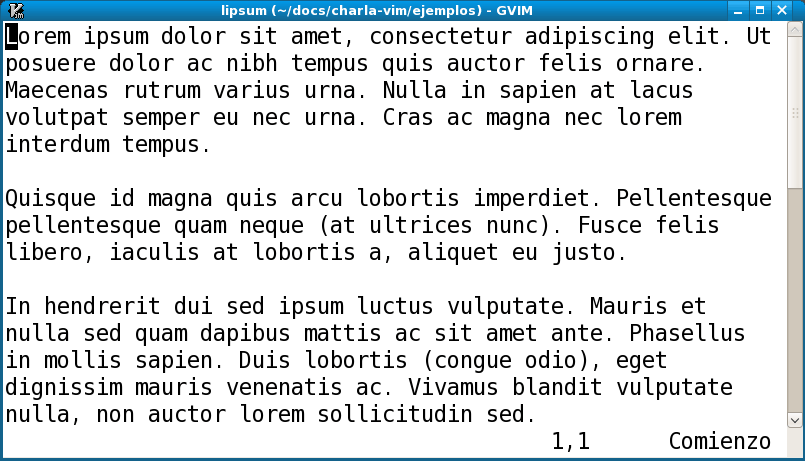
\includegraphics[width=\textwidth]{capturas/mov-01-nq8}}
    \only<2>{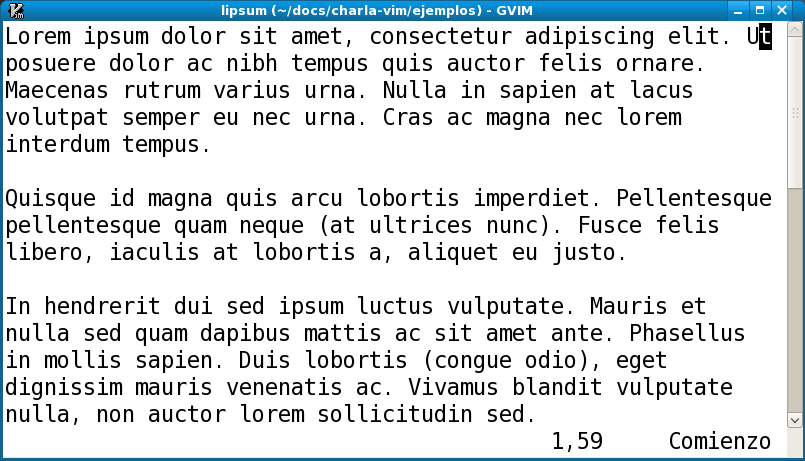
\includegraphics[width=\textwidth]{capturas/mov-02-nq8}}
    \only<3>{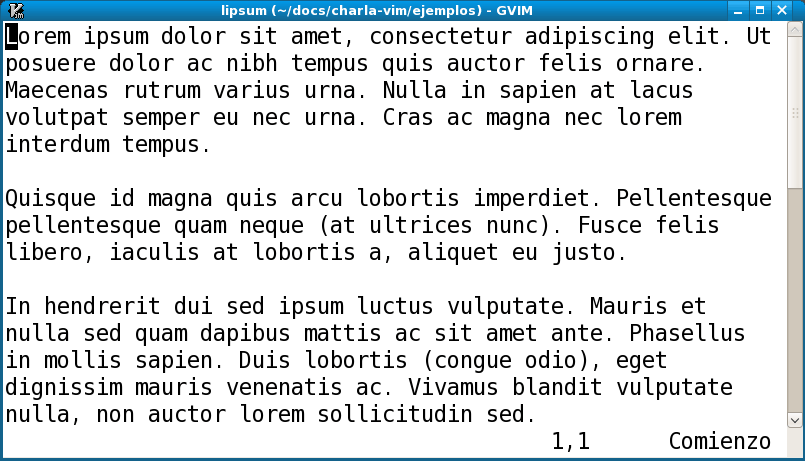
\includegraphics[width=\textwidth]{capturas/mov-03-nq8}}
    \only<4>{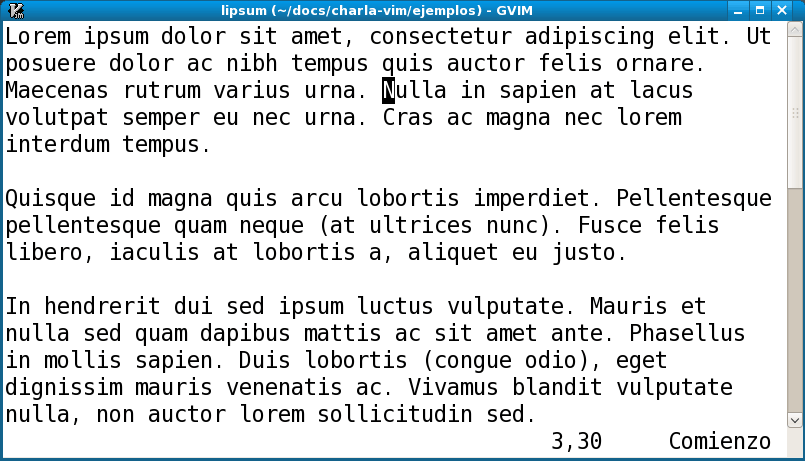
\includegraphics[width=\textwidth]{capturas/mov-04-nq8}}
    \only<5>{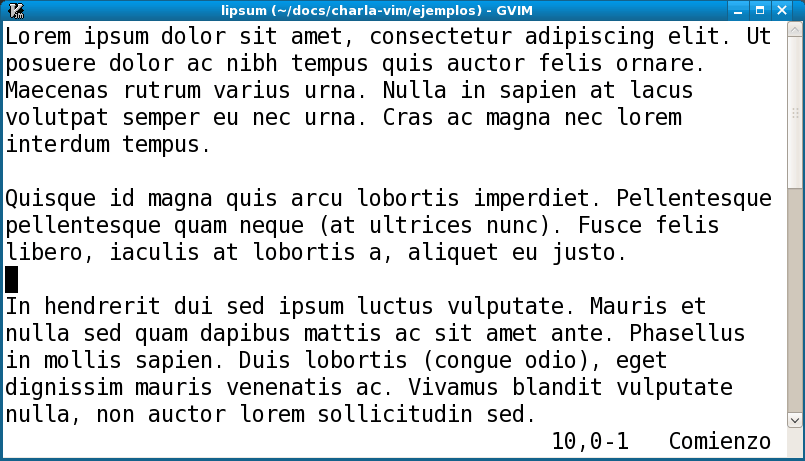
\includegraphics[width=\textwidth]{capturas/mov-05-nq8}}
    \only<6>{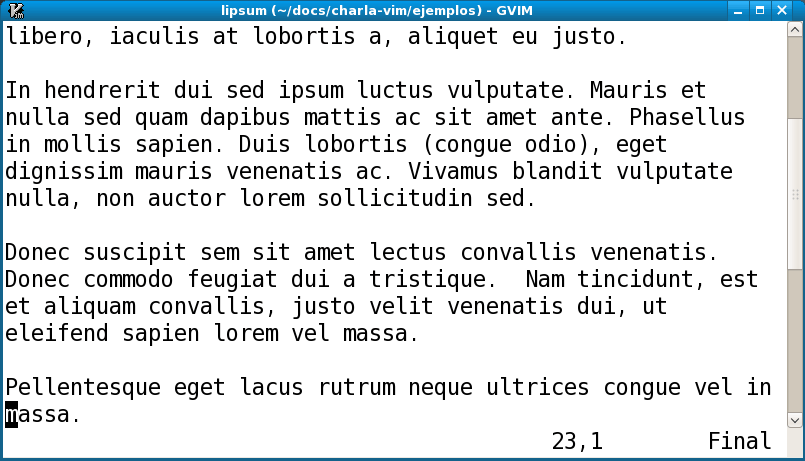
\includegraphics[width=\textwidth]{capturas/mov-06-nq8}}
    \only<7>{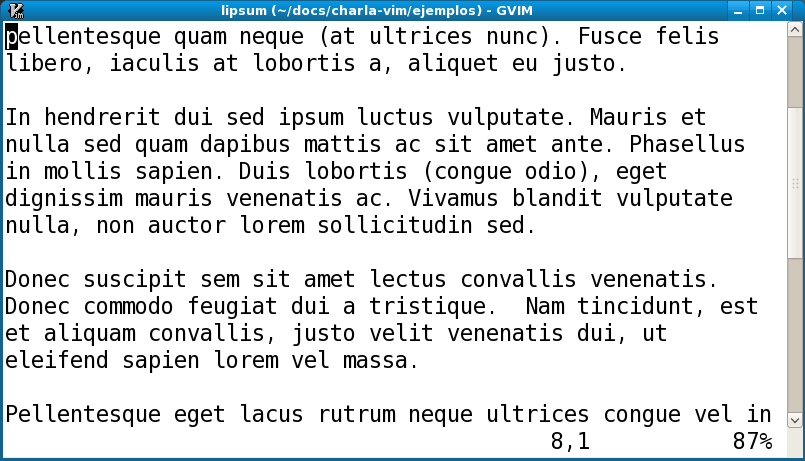
\includegraphics[width=\textwidth]{capturas/mov-07-nq8}}
    \only<8>{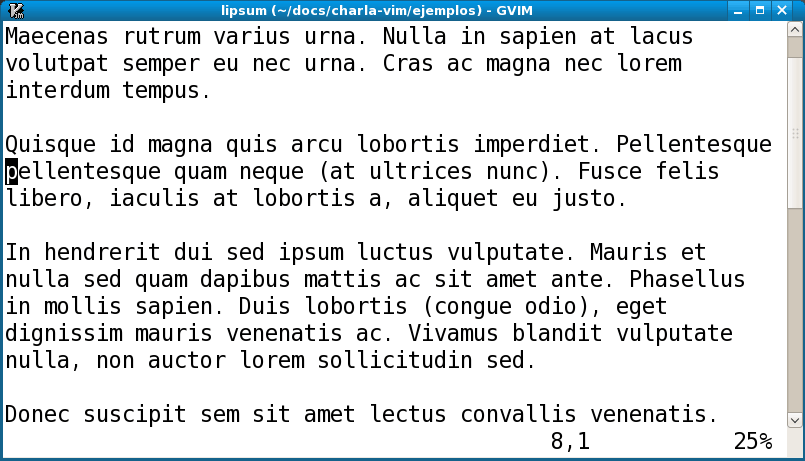
\includegraphics[width=\textwidth]{capturas/mov-08-nq8}}
    \only<9>{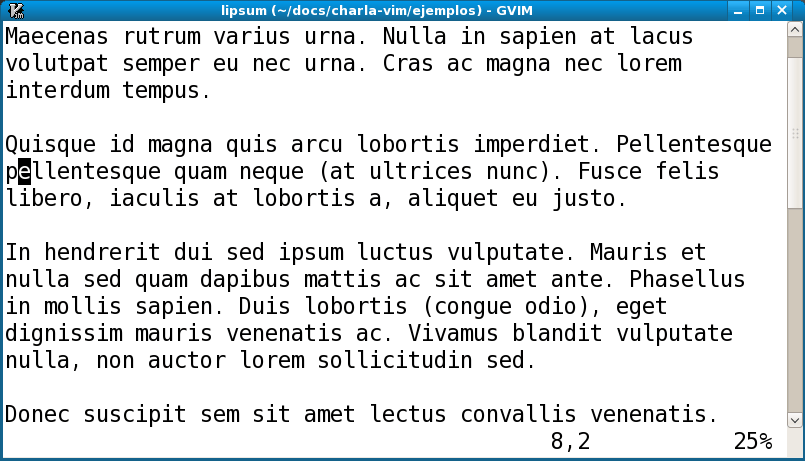
\includegraphics[width=\textwidth]{capturas/mov-09-nq8}}
    \only<10>{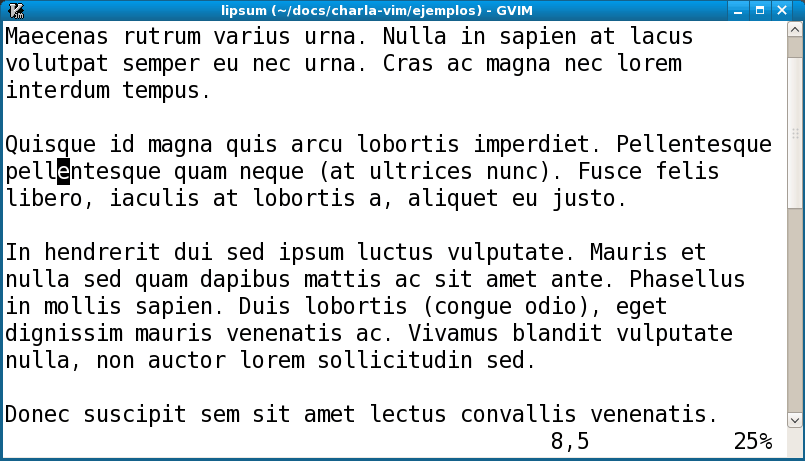
\includegraphics[width=\textwidth]{capturas/mov-10-nq8}}
    \only<11>{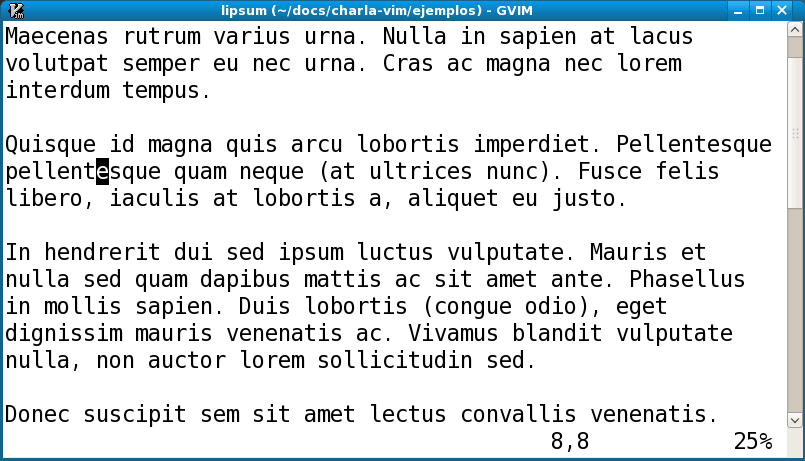
\includegraphics[width=\textwidth]{capturas/mov-11-nq8}}
    \only<12>{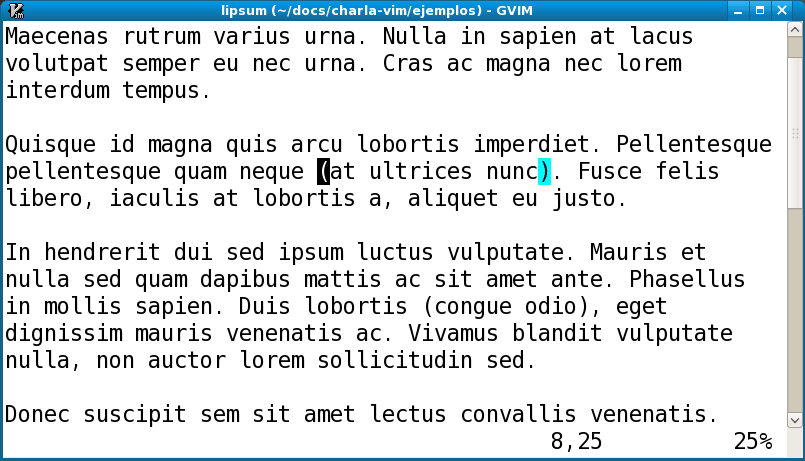
\includegraphics[width=\textwidth]{capturas/mov-12-nq8}}
    \only<13>{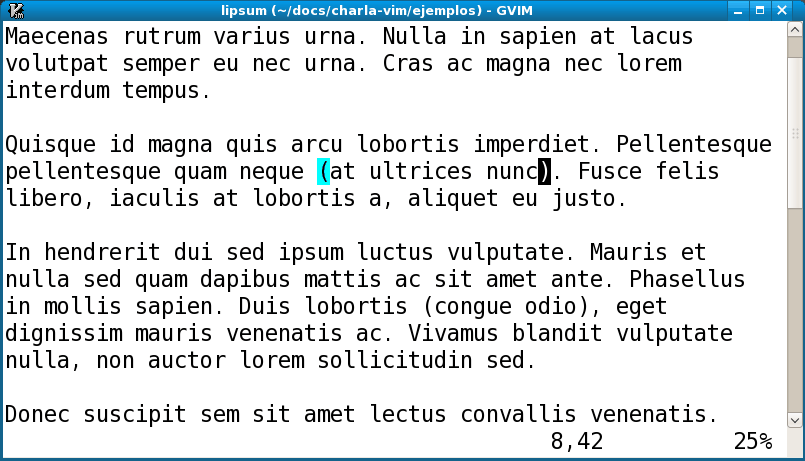
\includegraphics[width=\textwidth]{capturas/mov-13-nq8}}
    \only<14>{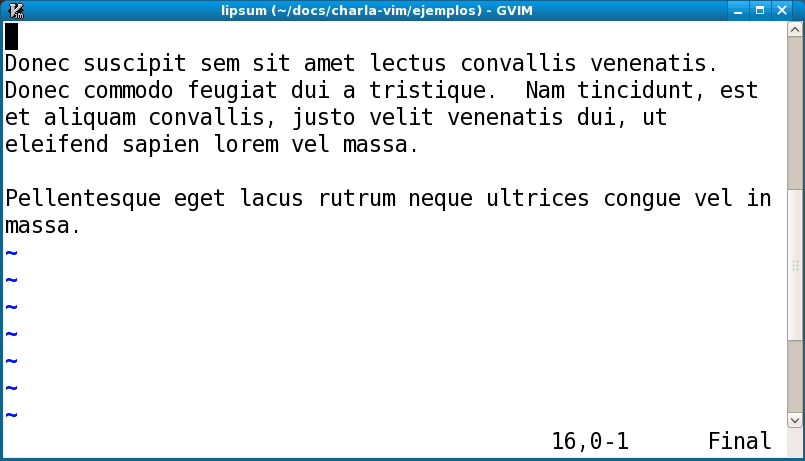
\includegraphics[width=\textwidth]{capturas/mov-14-nq8}}
    \only<15>{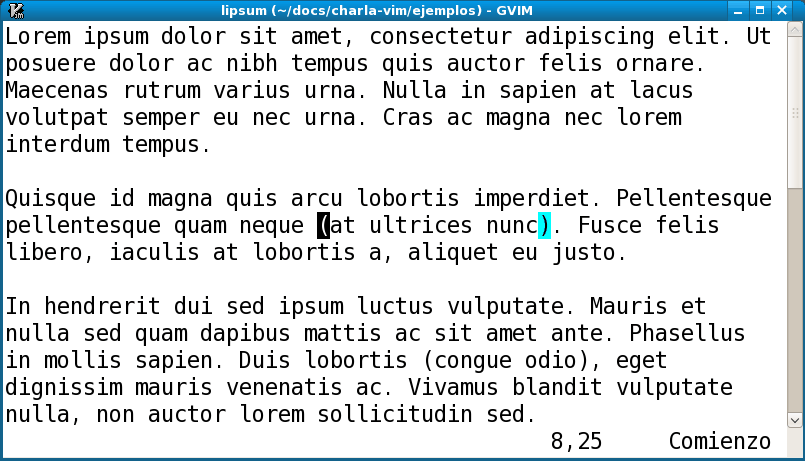
\includegraphics[width=\textwidth]{capturas/mov-15-nq8}}
    \only<16>{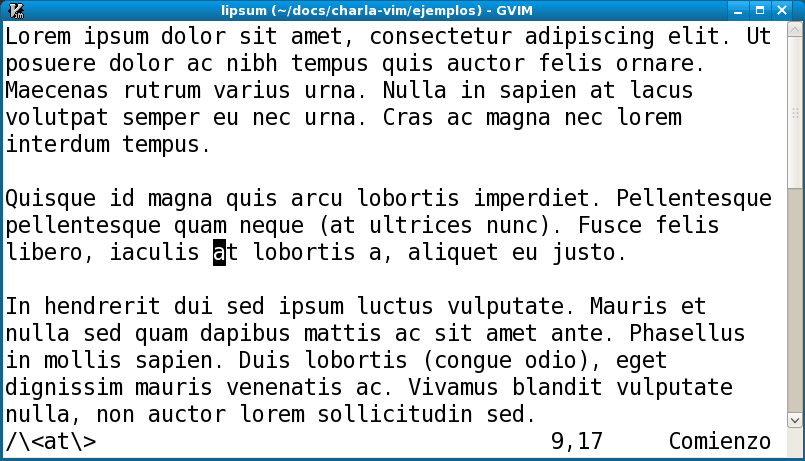
\includegraphics[width=\textwidth]{capturas/mov-16-nq8}}
    \only<17>{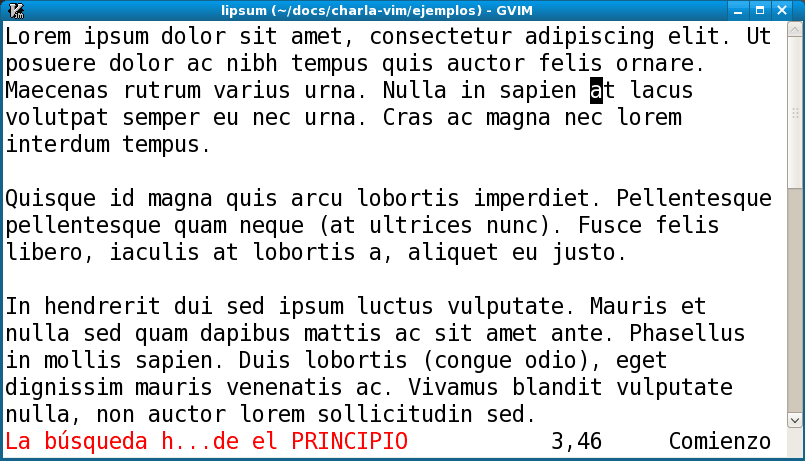
\includegraphics[width=\textwidth]{capturas/mov-17-nq8}}
    \uncover<2->{\key{\$}}
    \uncover<3->{\key{0}}
    \uncover<4->{\key{3}\key{$)$}}
    \uncover<5->{\key{2}\key{$\}$}}
    \uncover<6->{\key{G}}
    \uncover<7->{\key{8}\key{g}\key{g}}
    \uncover<8->{\key{5}\longkey{Ctrl Y}} \\
    \uncover<9->{\key{f}\key{e}}
    \uncover<10->{\key{;}}
    \uncover<11->{\key{;}}
    \uncover<12->{\key{3}\key{w}}
    \uncover<13->{\key{\%}}
    \uncover<14->{\longkey{Ctrl F}}
    \uncover<15->{\longkey{Ctrl O}}
    \uncover<16->{\key{*}}
    \uncover<17->{\key{n}}
\end{frame}

%  \item \key{\%}, \key{$*$}, \key{\#}
%  \item \key{`}\anykey, \key{'}\anykey
%  \item \longkey{Ctrl O}, \longkey{Ctrl I}
%  \item \key{H}, \key{M}, \key{L}

\begin{frame}
    \frametitle{Movimientos}
    \framesubtitle{Movimientos del contenido de la pantalla}
    \begin{itemize}
        \item \longkey{Ctrl F}: desplaza una página hacia adelante
            (\foreign{forwards})
        \item \longkey{Ctrl B}: desplaza una página hacia atras
            (\foreign{backwards})
        \item \longkey{Ctrl E}: desplaza una línea hacia arriba
            (\foreign{extra lines})
        \item \longkey{Ctrl Y}: desplaza una línea hacia abajo
        \item \key{z}\key{z}: deja la línea actual en el centro de la pantalla
    \end{itemize}
\end{frame}

\begin{frame}
    \frametitle{Movimientos}
    \framesubtitle{Movimientos relativos a la pantalla}
    \begin{itemize}
        \item \key{H}: mueve el cursor a la primera línea de la pantalla
            (\foreign{higher})
        \item \key{M}: mueve el cursor a la línea del medio de la pantalla
            (\foreign{middle})
        \item \key{L}: mueve el cursor a la última línea de la pantalla
            (\foreign{lower})
    \end{itemize}
\end{frame}

\begin{frame}
    \frametitle{Movimientos}
    \framesubtitle{Movimientos por línea}
    \begin{itemize}
        \item \key{g}\key{g}: mueve el cursor a la primera línea del archivo
            %(\foreign{go, go!})
        \item \key{G}: mueve el cursor a la última línea del archivo
            %(\foreign{GO!})
        \item \cmdcount\key{g}\key{g}: mueve  el cursor a la línea \cmdcount.
        \item \cmdcount\key{G}: ídem
        \item \cmdcount\key{\%}: mueve el cursor a la línea correspondiente al
            \cmdcount\ porciento de las líneas del archivo
    \end{itemize}
\end{frame}

\begin{frame}
    \frametitle{Movimientos}
    \framesubtitle{Movimientos por objetos de texto}
    \begin{itemize}
        \item \key{$($}, \key{$)$}: movimiento por oración
        \item \key{$\{$}, \key{$\}$}: movimiento por párrafo
    \end{itemize}
\end{frame}

\begin{frame}
    \frametitle{Movimientos}
    \framesubtitle{Movimientos en una línea}
    \begin{itemize}
        \item \key{0}:  principio de la línea
        \item \key{\$}:  final de la línea
        \item \key{$\wedge$}: primer caracter no blanco
        \item \key{f}\anykey: próxima ocurrencia de \anykey{} en la línea
            (\foreign{find})
        \item \key{F}\anykey: anterior ocurrencia de \anykey{} en la línea
        \item \key{t}\anykey: un caracter antes del próximo \anykey{}
            (\foreign{`til})
        \item \key{T}\anykey: un caracter después del anterior \anykey{}
        \item \key{;}: repite el último \key{f}, \key{F}, \key{t} o \key{T}.
    \end{itemize}
\end{frame}

\begin{frame}
    \frametitle{Movimientos}
    \framesubtitle{Otros movimientos}
    \begin{itemize}
        \item \key{\%}: busca el paréntesis apareado con el que está bajo el
            cursor 
            \begin{itemize}
                \item funciona para
                    \texttt{()},
                    \texttt{\{\}},
                    \texttt{[]},
                    \texttt{\#if \#endif},
                    \texttt{/* */}.
            \end{itemize}
        \item \longkey{Ctrl O}: retorna a la posición anterior antes del último
            movimiento (\foreign{old position})
        \item \longkey{Ctrl I}: deshace el \longkey{Ctrl O}
    \end{itemize}
\end{frame}

\begin{frame}
    \frametitle{Operaciones básicas}
    \begin{itemize}
        \item \key{$\sim$}:  cambia minúsculas/mayúsculas del caracter bajo el
            cursor
        \item \key{x}:  suprime el caracter bajo el cursor
        \item \key{X}:  suprime el caracter anterior al cursor
        \item \key{r}\anykey:  reemplaza el caracter bajo el cursor por \anykey
        %\item \key{m}\anykey
        \item \longkey{Ctrl A}:  incrementa el número bajo el cursor
            (\foreign{add})
        \item \longkey{Ctrl X}:  decrementa el número bajo el cursor
            (\foreign{extract})
        %\item \key{u}: deshace el último comando (\foreign{undo})
        %\item \key{.}: repite el último comando
    \end{itemize}
\end{frame}

\begin{frame}
    \frametitle{¿Cómo comenzar a escribir?}
    \begin{itemize}
        \item \key{i}:  comienza a escribir antes del cursor (\foreign{insert})
        \item \key{s}:  comienza a escribir encima del cursor
            (\foreign{substitute})
        \item \key{a}:  comienza a escribir después del cursos
            (\foreign{append})
        \item \key{I}:  comienza a escribir al principio de la línea
        \item \key{A}:  comienza a escribir al final de la línea
        \item \key{o}:  comienza a escribir en una línea nueva a continuación
            de la actual (\foreign{open new line})
        \item \key{O}:  comienza a escribir en una línea nueva antes de la
            actual
        \item<2> Al terminar de escribir, presionar \longkey{Esc}
    \end{itemize}
\end{frame}

\begin{frame}
    \frametitle{Comandos paltosos en modo inserción}
    \begin{itemize}
        \item \longkey{Ctrl H}, \longkey{Ctrl U}: borra el caracter
            anterior/hasta el final de la línea
        \item \longkey{Ctrl T}, \longkey{Ctrl D}: indenta/dedenta la línea
            actual
        \item \longkey{Ctrl Y}, \longkey{Ctrl E}: copia el caracter arriba/abajo
            del cursor
        \item \longkey{Ctrl P}, \longkey{Ctrl N}: completa la palabra que se
            está escribiendo
        \item \longkey{Ctrl X}\longkey{Ctrl F}, \longkey{Ctrl X}\longkey{Ctrl L}
    \end{itemize}
\end{frame}

\begin{frame}
    \frametitle{Operadores}
    \begin{itemize}
        \item \key{c}\cmd{mov}, \key{d}\cmd{mov}, \key{y}\cmd{mov}
        \item \key{g}\key{$\sim$}\cmd{mov}, \key{g}\key{u}\cmd{mov},
            \key{g}\key{U}\cmd{mov}
        \item \key{!}\cmd{mov}, \key{=}\cmd{mov}, \key{g}\key{q}\cmd{mov},
            \key{g}\key{?}\cmd{mov}
        \item \key{$>$}\cmd{mov}, \key{$<$}\cmd{mov}
        \item Comando repetido se aplica a la línea actual
    \end{itemize}
\end{frame}

\begin{frame}
    \frametitle{Ejemplos de uso de operadores}
    \begin{itemize}
        \item \key{c}\key{w}\typed{lala}\longkey{Esc}
        \item \key{b}\key{y}\key{\$}\key{0}\key{P}
        \item \key{d}\key{d}\key{p} 
        \item \key{g}\key{g}\key{O}\typed{\#include
            "lala.h"}\longkey{Esc}\longkey{Ctrl O}
        \item \longkey{Ctrl A}\key{2}\key{j}\key{.}
        \item \key{I}\typed{/$*$}\longkey{Esc}\key{A}\typed{$*$/}\longkey{Esc}
        \item \key{F}\key{$\{$}\key{d}\key{\%}\key{20}\key{k}\key{p}
    \end{itemize}
\end{frame}

\begin{frame}
    \frametitle{Ejemplos de operadores con pseudomovimientos}
    \begin{itemize}
        \item \key{d}\key{i}\key{w}
        \item \key{g}\key{q}\key{a}\key{p}
        \item \key{c}\key{i}\key{$\}$}\typed{Blah blah}\longkey{Esc}
    \end{itemize}
\end{frame}

\begin{frame}
    \frametitle{Modo visual}
    \begin{itemize}
        \item \key{v}: selección por caracteres
        \item \key{V}: selección por líneas
        \item \longkey{Ctrl V}: selección en bloque
    \end{itemize}
\end{frame}

\begin{frame}
    \frametitle{Modo ex (línea de comandos)}
    \begin{itemize}
        \item \key{:}\typed{e \placeholder{archivo}}\longkey{Enter}
        \item \key{:}\typed{w \placeholder{archivo}}\longkey{Enter}
        \item \key{:}\typed{w}\longkey{Enter}
        \item \key{:}\typed{3,\$w}\longkey{Enter}
        \item \key{:}\typed{wq}\longkey{Enter}
        \item \key{:}\typed{r  \placeholder{archivo}}\longkey{Enter}
        \item \key{:}\typed{r! \placeholder{comando}}\longkey{Enter}
    \end{itemize}
\end{frame}

\begin{frame}
    \frametitle{Modo ex, segunda parte}
    \begin{itemize}
        \item \key{:}\typed{.,+5d}\longkey{Enter}
        \item \key{:}\typed{2,\$normal 02fñx\$}\longkey{Enter}
        \item
            \key{:}\typed{\%s/textbf/emph/gc}\longkey{Enter}
        \item \key{:}\typed{g/item/d}\longkey{Enter}
            \key{:}\typed{g/$\wedge$[ ]$*$\#/normal A \#XXX}\longkey{Enter}
        \item \key{:}\typed{1,.j}\longkey{Enter}
    \end{itemize}
\end{frame}

\begin{frame}
    \frametitle{Búsqueda}
    \begin{itemize}
        \item \key{/}\typed{\placeholder{patrón}}\longkey{Enter}: busca el
            patrón hacia adelante
        \item \key{?}\typed{\placeholder{patrón}}\longkey{Enter}: busca el
            patrón hacia atrás
        \item \key{n}, \key{N}: busca próxima/anterior ocurrencia de la última
            búsqueda
        \item \key{$*$}, \key{\#}: busca próxima/anterior ocurrencia de la
            palabra bajo el cursor
    \end{itemize}
\end{frame}

\begin{frame}
    \frametitle{Mapeos y abreviaciones}
    \begin{itemize}
        \item \key{:}\typed{map \placeholder{secuencia} \placeholder{secuencia}}\longkey{Enter}
        \item \key{:}\typed{imap \placeholder{secuencia} \placeholder{secuencia}}\longkey{Enter}
        \item \key{:}\typed{noremap \placeholder{secuencia} \placeholder{secuencia}}\longkey{Enter}
        \item \key{:}\typed{iabbrev \placeholder{abreviación} \placeholder{texto}}\longkey{Enter}
    \end{itemize}
\end{frame}

\begin{frame}
    \frametitle{Macros}
    \begin{itemize}
        \item \key{q}\anykey: comienza a grabar una macro en el registro \anykey
        \item \key{@}\anykey: ejecuta la macro grabada en \anykey
        \item \key{@}\key{@}: ejecuta la última macro ejecutada
    \end{itemize}
\end{frame}

\begin{frame}
    \frametitle{Ventanas}
    \begin{itemize}
        \item \key{:}\typed{new}\longkey{Enter}
        \item \key{:}\typed{vnew}\longkey{Enter}
        \item \longkey{Ctrl W}\key{n}
        \item \longkey{Ctrl W}\longkey{Ctrl W}
        \item \longkey{Ctrl W}\key{j},\longkey{Ctrl W}\key{l}
        \item \longkey{Ctrl W}\key{J},\longkey{Ctrl W}\key{L}
    \end{itemize}
\end{frame}

\end{document}
